\documentclass{article}

\usepackage{graphicx, hyperref, cleveref, cite, epstopdf}

\title{CS 6660: Scaling Projective Dynamics on GPU}
\author{Will Usher and Pavol Klacansky}

\begin{document}
\maketitle

\section{Introduction}
Projective Dynamics~\cite{Bouaziz14} solves a continuum mechanics system using
a local projective step and global implicit solver step. The local step independently
projects each constraint to its desired constrained state and is easy to parallelize.
The global step solves a system of linear equations which represent
the projections and external forces (including inertia). We choose to explore
parallelization of the global step since the local step is trivial (we do
parallelize the local step as well), by implementing
a special case of projective dynamics for mass-spring systems~\cite{Liu13}

\section{Direct Solvers}
Direct solvers are difficult to parallelize due interdependencies and we
expected low performance on the GPU. We used cuSPARSE to solve the global step and it
was significantly slower than conjugate gradient on the GPU via ViennaCL,
see Figure~\ref{fig:cusparse_vs_cg}.

\begin{figure}[htb!]
	\centering
	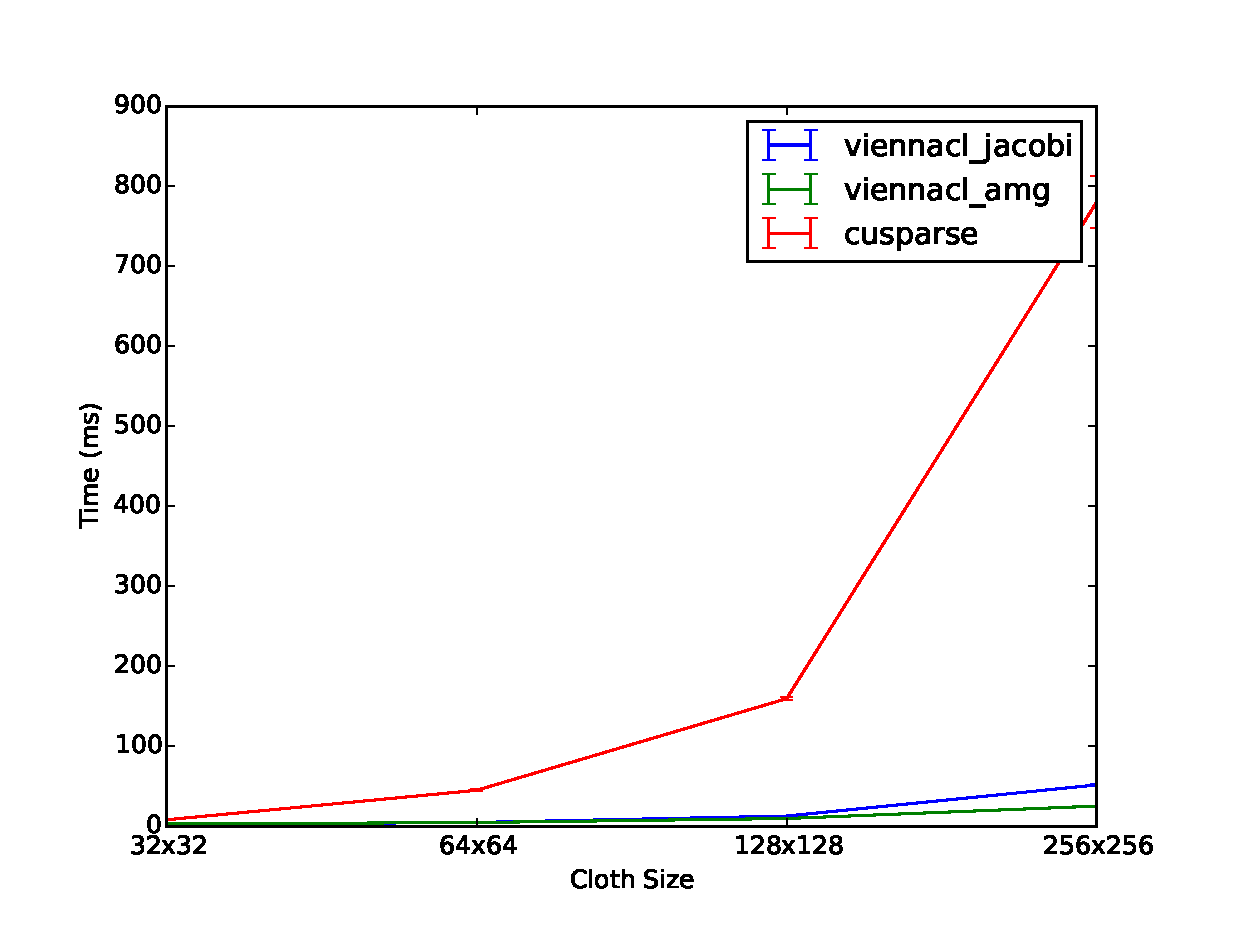
\includegraphics[width=0.9\linewidth]{img/cusparse_vs_cg}
	\caption{Comparing cuSPARSE's direct GPU solver with ViennaCL's conjugate gradient
		solver. \label{fig:cusparse_vs_cg}}
\end{figure}

\section{Iterative Solvers}
The global system matrix we're solving is SPD, so we tried the conjugate gradient
solver from the ViennaCL library with various preconditioners. From our tests,
after certain size (256x256) the algebraic multigrid preconditioner outperforms Jacobi
or no preconditioning, see Figure~\ref{fig:viennacl_preconds}.

The state-of-the art iterative solver seems to be~\cite{Wang15} and we tried
to implement it but we could not get it working. Another pitfall of this method
is that it has many input parameters to set up and tweak.

\begin{figure}[htb!]
	\centering
	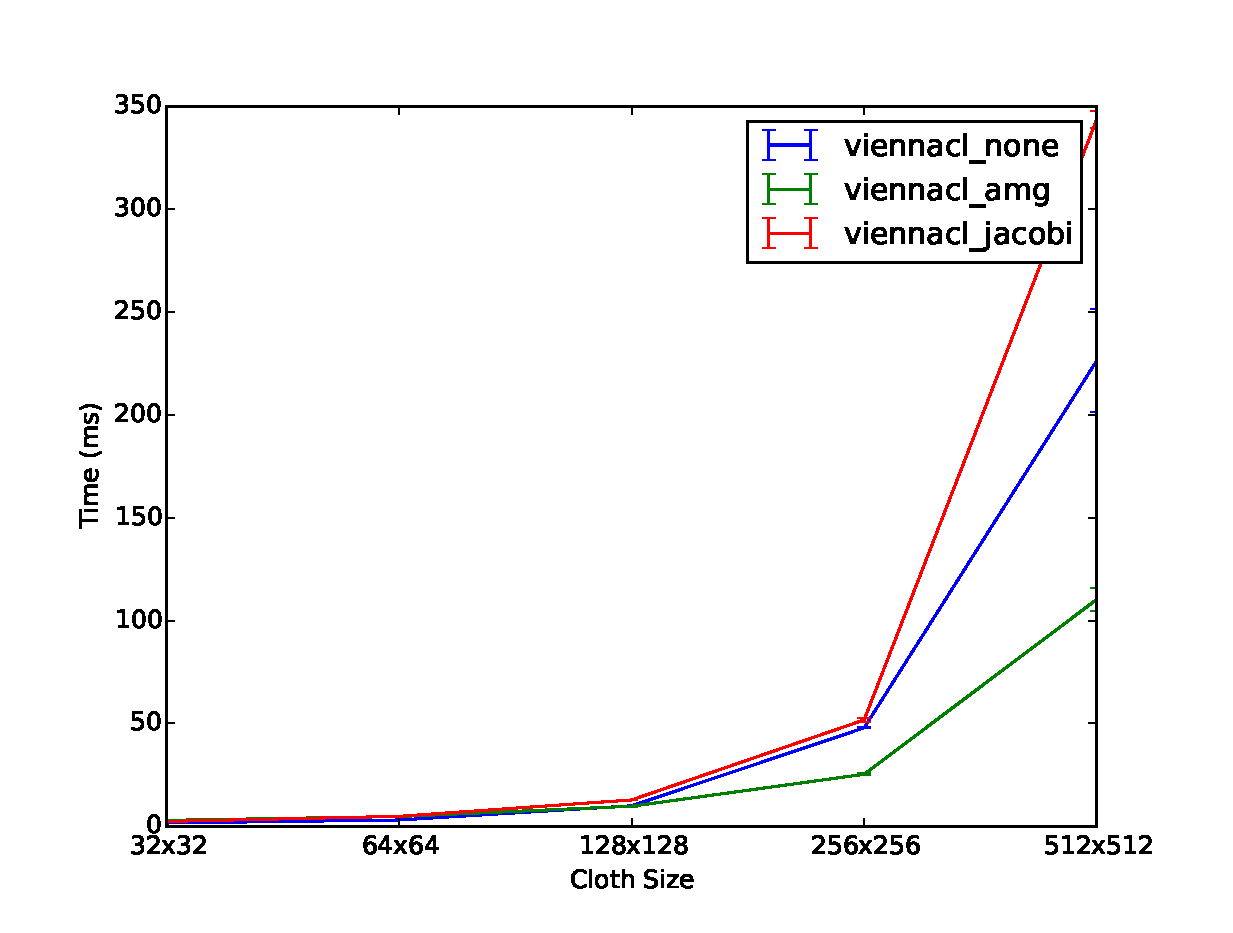
\includegraphics[width=0.9\linewidth]{img/viennacl_none_jacobi_amg}
	\caption{ViennaCL CUDA CG solver with different preconditioners.
	\label{fig:viennacl_preconds}}
\end{figure}

\begin{figure}[htb!]
        \centering
		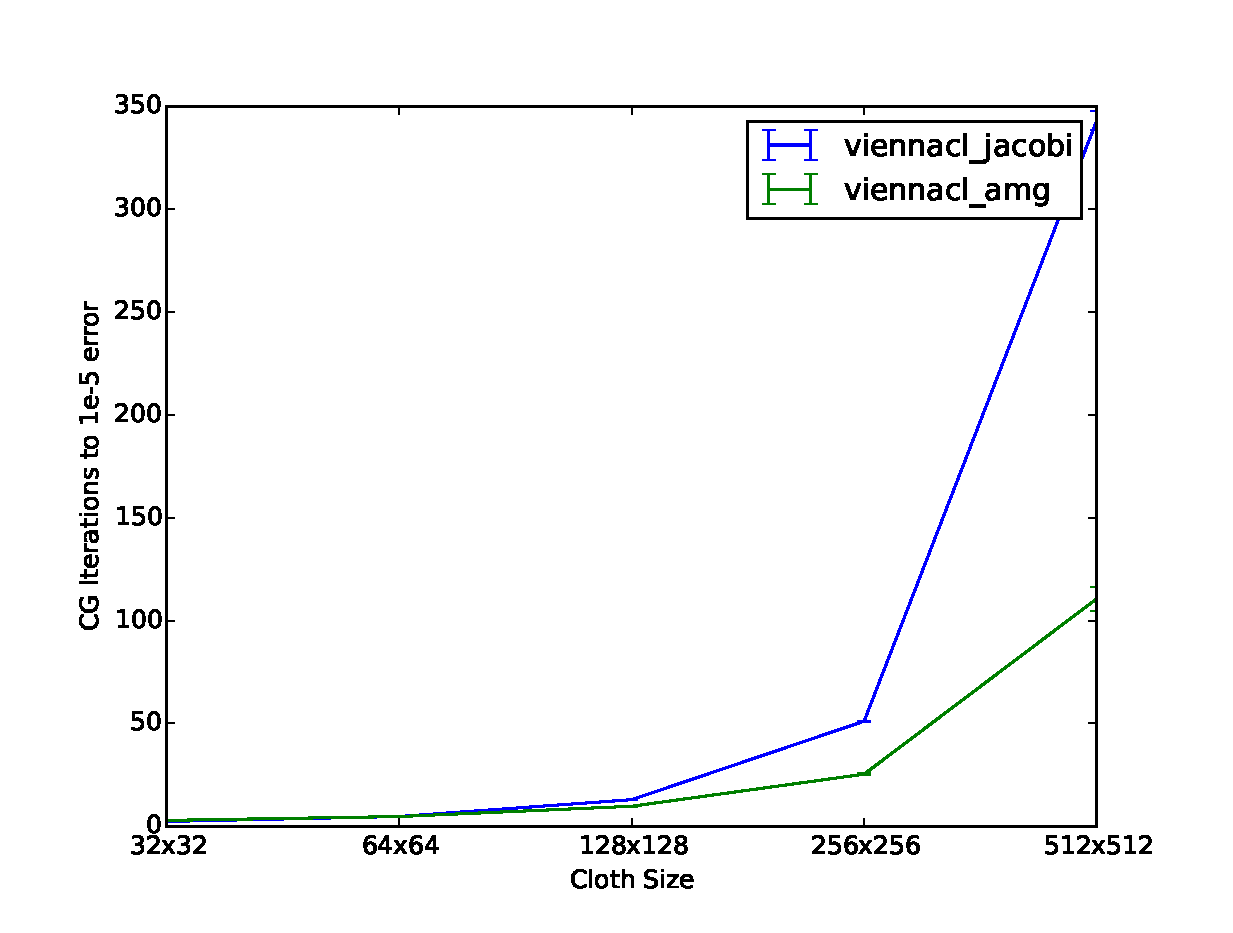
\includegraphics[width=0.9\linewidth]{img/amg_vs_jacobi_iters}
		\caption{Number of iterations required to converge to $1 \times 10^{-5}$ error with ViennaCL's
			conjugate gradient solver. \label{fig:amg_vs_jacobi_iters}}
\end{figure}

\section{Domain Decomposition}
In previous sections we noted that direct solvers are mostly serial (PARDISO
was getting less than 2x speedup on 4 cores with 8 HW threads). We also tried
a block Jacobi solver with Eigen's SimplicialLLT direct solver for each diagonal
scaled rather poorly, Figure~\ref{fig:block_jacobi_scaling}. We think
the scaling is affected by limited memory bandwidth and load imbalance, as
the columns in the individual rows are executed in serial.


\begin{figure}[htb!]
	\centering
	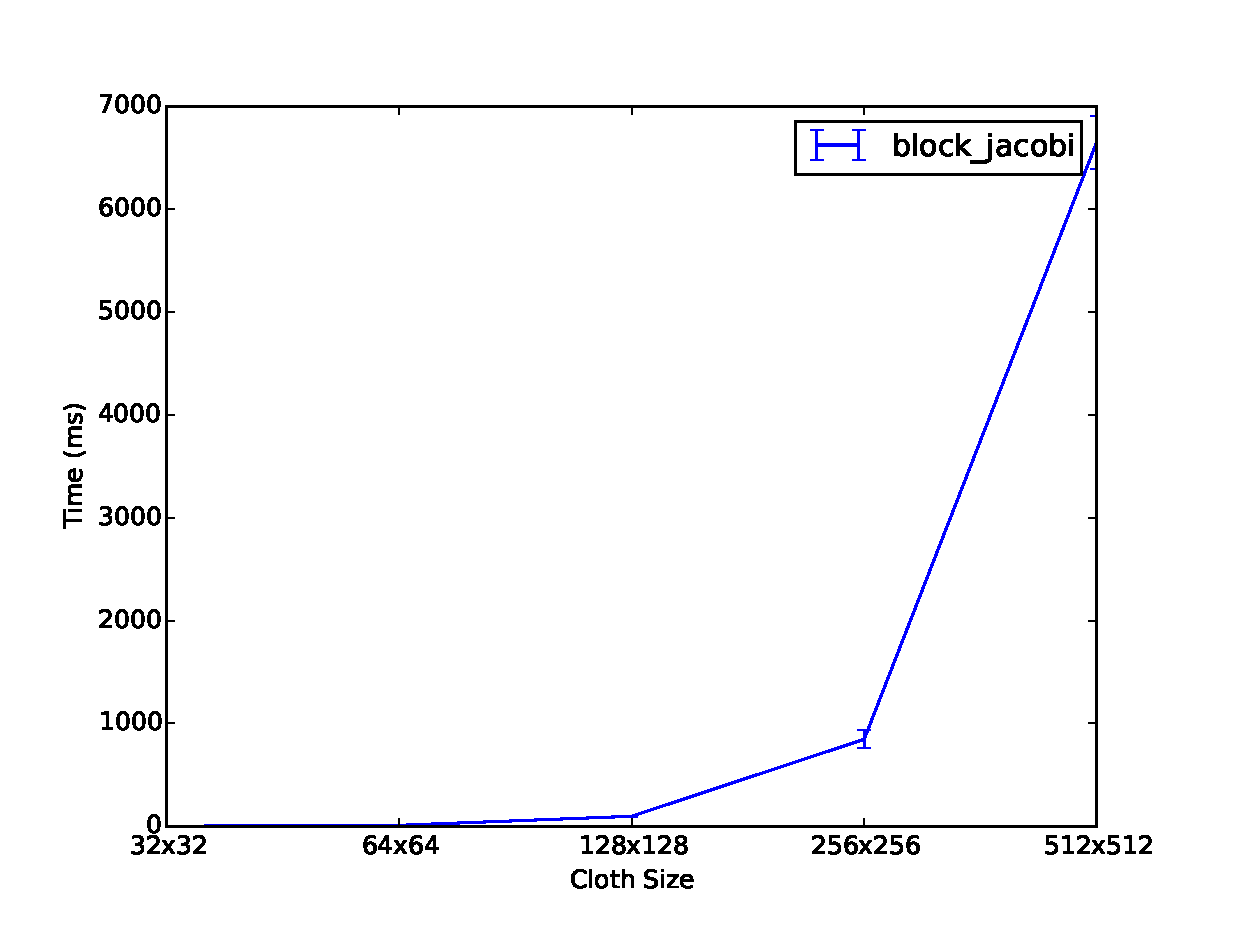
\includegraphics[width=0.9\linewidth]{img/block_jacobi_scaling}
	\caption{Block Jacobi scaling on a CPU with 12 cores using 12 blocks.
	\label{fig:block_jacobi_scaling}}
\end{figure}

We also tested some basic (incorrect) domain decompositions, one where two
pieces of cloth overlap and each acts as attachment constraint for the other.
This approach is data parallel as the attachments are updated after both
cloths were solved.

The other approach is to use a third cloth to glue the two pieces and do a
fan-in (i.e. solve two pieces in parallel, then solve middle piece). We did
not set the vertex weights properly and are unsure on what weights would be right,
thus our cloth exploded as the middle step inserts energy by pulling too much on
the left and right pieces being connected.

\section{Conclusion}
During this project we have explored direct and iterative solvers on GPU,
simple domain decompositions, and a parallel block Jacobi solver on the CPU.
Figure~\ref{fig:amg_direct} compares the best performing solver on the CPU and
GPU. We found that iterative solvers do not perform well in PD, as the
timestep gets larger the iteration count increases sublinearly, thus the
direct solver will eventually outperform the iterative solver.

\begin{figure}[htb!]
        \centering
        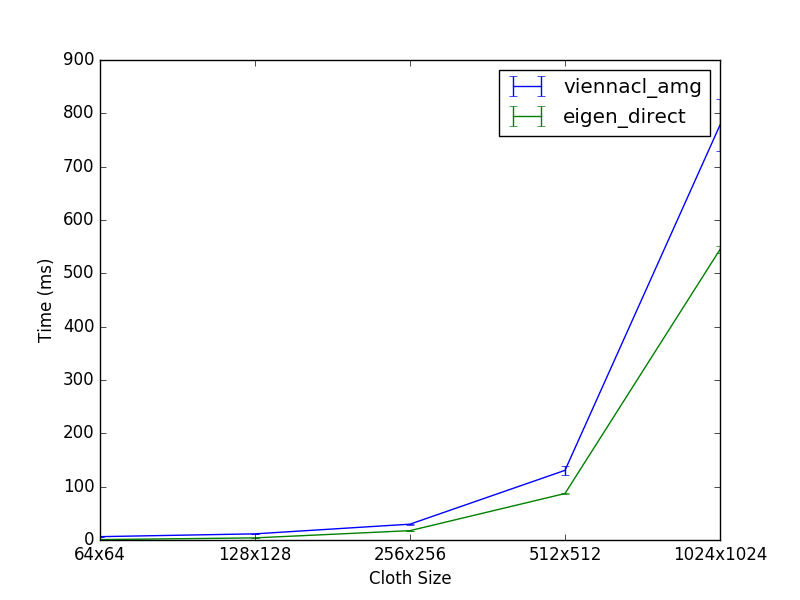
\includegraphics[width=0.9\linewidth]{img/amg_direct.png}
        \caption{Direct solver on CPU compares to CG with AMG preconditioner
                 on GPU. \label{fig:amg_direct}}
\end{figure}

We conclude the best performing solver is the Chebyshev approach by Wang~\cite{Wang15},
which outperforms both single core direct solver (1.5x) and AMG CG on GPU (3x).
Unfortunately, we tried and failed to get it working in our framework, thus
the comparison is based only on number of points ($L$ matrix). The major
downside of Chebyshev method is many tweakable parameters which need
to be tuned for the simulation.

\bibliography{report}{}
\bibliographystyle{plain}

\end{document}
